% begin module tangents-ex2
\begin{frame}
\begin{example} %[Example 2, p. 136]
\begin{columns}[c]
\column{.55\textwidth}
Find an equation for the tangent line to the hyperbola $y = 3/x$ at the point $(3,1)$.

\psset{xunit=0.6cm, yunit=0.6cm}
\begin{pspicture}(-5, -5)(5,5) 
\psframe*[linecolor=white](-5,-10)(5,10) 
\psaxes[ticks=none, labels=none]{<->}(0,0)(-5,-3)(5,5)
%Function formula: (3)/(x) 
\psplot[linecolor=red, plotpoints=1000]{0.6}{5}{3 x div } %Function formula: (3)/(x) 
\psplot[linecolor=red, plotpoints=1000]{-5}{-1}{3 x div }
\rput(2.2, 3){$y=\frac{3}{x}$}

\uncover<9->{
\psline[linecolor=blue](-5, 3.666666667)(5, 0.333333333)
\rput(-2.5, 4){$x+3y-6=0$}
}
\psFullDotBlack{3}{1}
\rput[t](3, 0.8){\footnotesize $(3,1)$}
\end{pspicture} 
%\ \only<handout:0| -8>{%
%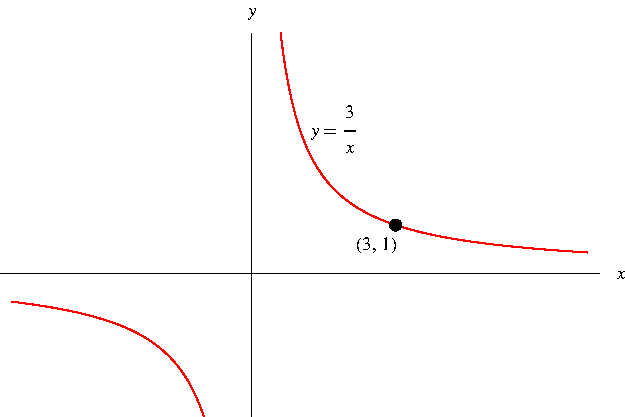
\includegraphics[height=4cm]{derivatives/pictures/03-01-ex2a.pdf}%
%}%
%\only<9->{%
%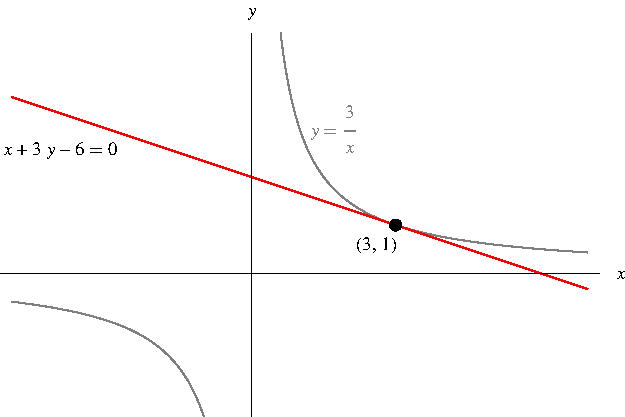
\includegraphics[height=4cm]{derivatives/pictures/03-01-ex2b.pdf}%
%}%

\uncover<9->{
Point-slope form: $y - 1 = -\frac{1}{3}(x - 3)$, or $x + 3y - 6 = 0$.
}
\column{.45\textwidth}
\uncover<2->{%
Here $a = 3$ and $f(x) = 3/x$.
}%
\abovedisplayskip=0pt
\belowdisplayskip=-15pt
\abovedisplayshortskip=0pt
\belowdisplayshortskip=0pt
\begin{align*}
\uncover<3->{m} & \uncover<3->{ = }  \uncover<3->{\lim_{h\rightarrow 0} \frac{f(3+ h)-f(3)}{h}}\\
& \uncover<4->{ = }  %
\uncover<4->{\lim_{h\rightarrow 0}\frac{\frac{3}{3+h} - 1}{h}}\\
& \uncover<5->{ = }  %
\uncover<5->{\lim_{h\rightarrow 0}\frac{\frac{3-(3+h)}{3+h}}{h}}\\
& \uncover<6->{ = }  %
\uncover<6->{\lim_{h\rightarrow 0}\frac{-h}{h(3+h)}}\\
& \uncover<7->{ = }  %
\uncover<7->{\lim_{h\rightarrow 0}-\frac{1}{3+h}}\uncover<9->{ = -\frac{1}{3}}
\end{align*}
\end{columns}
\end{example}
\end{frame}
% end module tangents-ex2
